Neste capítulo serão apresentadas as funcionalidades disponíveis aos usuários finais do sistema.
Deve ser possível emitir, visualizar, exportar e revogar um certificado digital.

Este capítulo, no entanto, não contém entradas específicas. Basta seguir o fluxo das atividades necessárias para emissão e revogação de certificado, observando se nenhum erro é apresentado e se as saídas se comportam da maneira esperada.

\section{Emissão de Certificado}

No menu \textit{Certificado} deve ser possível encontrar as ações de emitir e revogar.

Para emitir, é necessário selecionar a instituição na qual você é afiliado.  O usuário deve ser redirecionado para a tela de escolha de Federação, onde deve selecionar sua instituição. O usuário então deverá ser redirecionado para a página de autenticação da sua instituição, onde deve entrar com os dados do seu usuário já cadastrado. Os testes descritos aqui podem ser observados nas figuras \ref{fig:ufxc} e \ref{fig:ufxc2}.

\begin{figure}[ht]
     \centering
     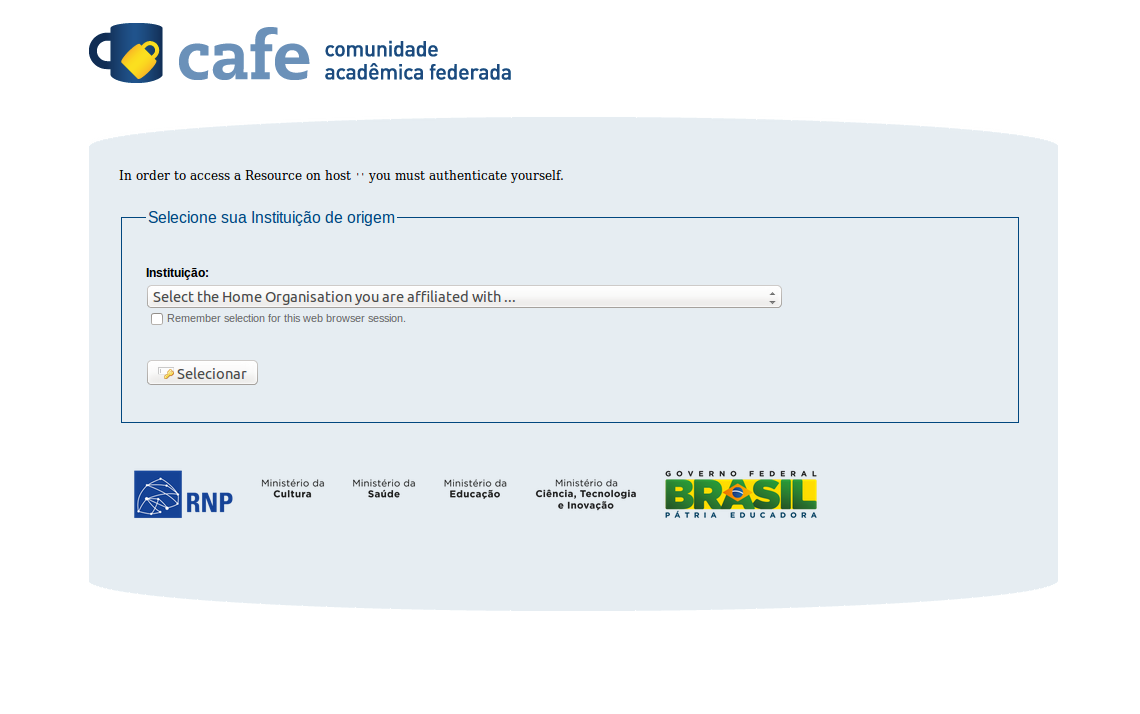
\includegraphics[scale=0.3]{images/escolher-federacao.png}
     \caption{Escolha de Federação}
     \label{fig:ufxc}
\end{figure}

\begin{figure}[ht]
     \centering
     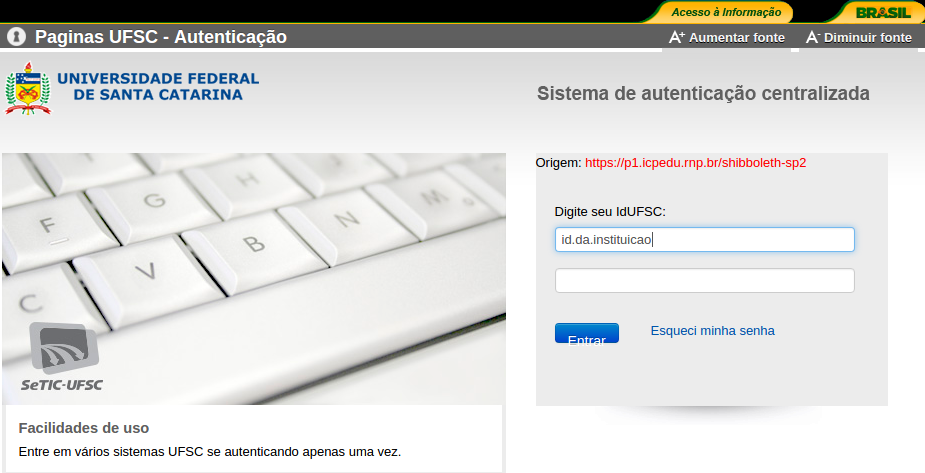
\includegraphics[scale=0.3]{images/emitir2.png}
     \caption{Autenticação na Federação}
     \label{fig:ufxc2}
\end{figure}

Se você já possui um certificado emitido nesta Autoridade Certificadora, e este ainda estiver ativo, um aviso deverá aparecer na tela informando que o certificado atual será revogado ao emitir um novo.

O usuário deverá ver uma tela com seus dados (Nome, CPF, E-mail e Data de  nascimento) já preenchidos, onde nenhum deles pode ser editado. Basta conferir os dados, escolher um tamanho de chave, uma senha para o arquivo PKCS\#12 e submeter a solicitação de certificado. Vide figura \ref{fig:emissao3}.

Quando o certificado for emitido, será apresentada a opção de fazer o download do arquivo no formato PKCS\#12. Os dados do certificado podem ser visualizados abrindo o arquivo e informando a senha escolhida. O arquivo PKCS\#12 pode ser importado no navegador. Ao visualizar, pelo navegador, o certificado digital emitido, deve ser possível conferir os dados gerais do certificado, em sua aba principal (imagem \ref{fig:geralcert}), e os detalhes do mesmo, em sua aba \textit{Details} (imagem \ref{fig:detailscert}).

\begin{figure}[ht]
     \centering
     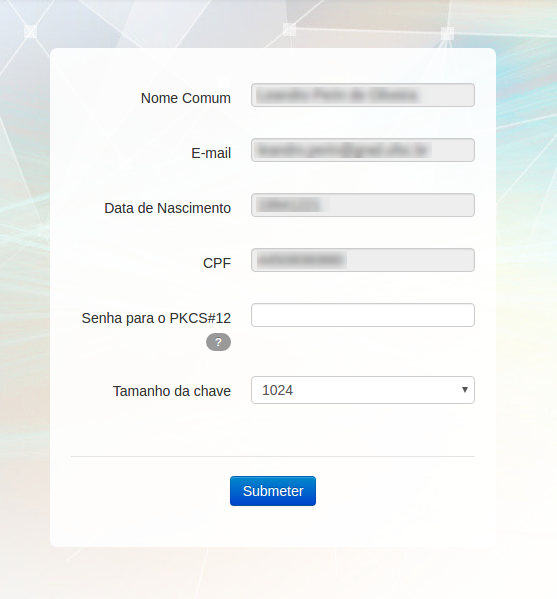
\includegraphics[scale=0.5]{images/firefox-solicitar-certificado.png}
     \caption{Confirmação de dados}
     \label{fig:emissao3}
\end{figure}

\begin{figure}[ht]
     \centering
     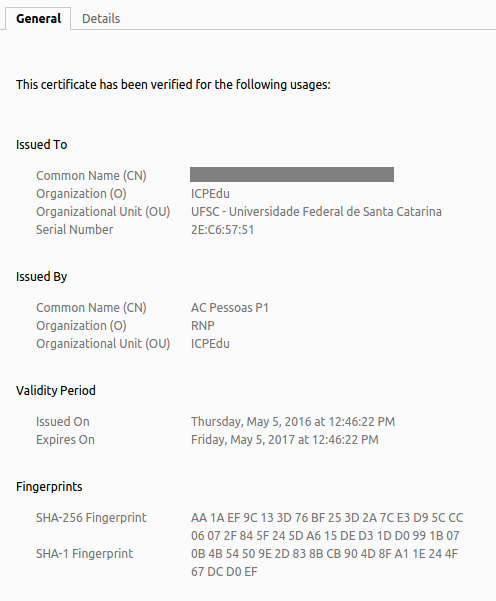
\includegraphics[scale=0.5]{images/geralcert.png}
     \caption{Informações gerais do certificado}
     \label{fig:geralcert}
\end{figure}

\begin{figure}[ht]
     \centering
     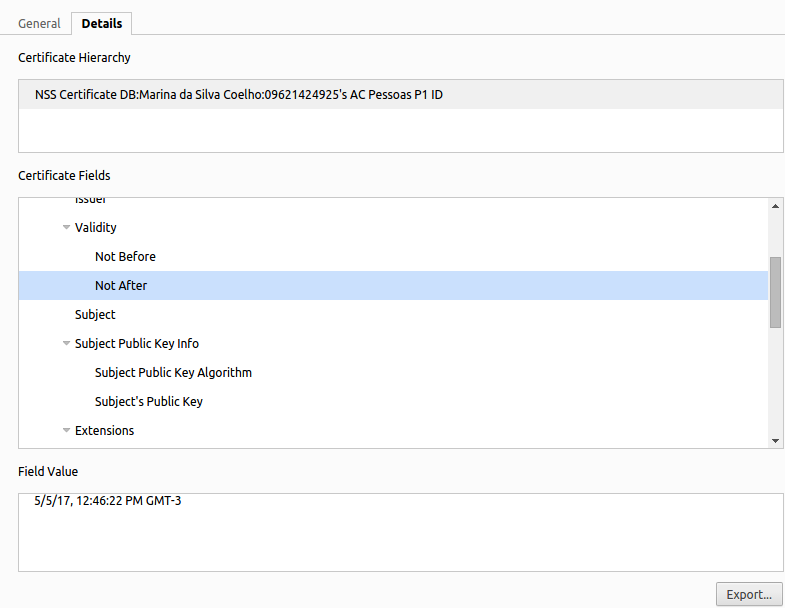
\includegraphics[scale=0.5]{images/details.png}
     \caption{Detalhes do certificado}
     \label{fig:detailscert}
\end{figure}

Como é possível ver na imagem \ref{fig:detailscert}, no canto inferior direito da tela de visualização de certificado, deve-se poder exportar o mesmo. A etapa para exportar o certificado envolve gerenciamento da chave do mesmo. Como este tipo de configuração é diferente para cada navegador (que também operam de maneira diferente dependendo do sistema operacional da máquina), o usuário deve se dirigir ao menu de ajuda, especificado na seção 6.2, onde deverá encontrar um guia detalhado de como exportar o certificado com base no navegador e sistema operacional utilizados no momento da exportação.

\section{Revogação de Certificado}

Para revogar, deve ser feito o mesmo processo de autenticação via federação necessário para a emissão, mostrado nas figuras \ref{fig:ufxc} e \ref{fig:ufxc2}. Os dados do certificado são então apresentados, e deve-se escolher o motivo de revogação, como mostra a figura \ref{fig:revoke}. Tendo escolhido este, deve-se clicar em submeter.

\begin{figure}[ht]
     \centering
     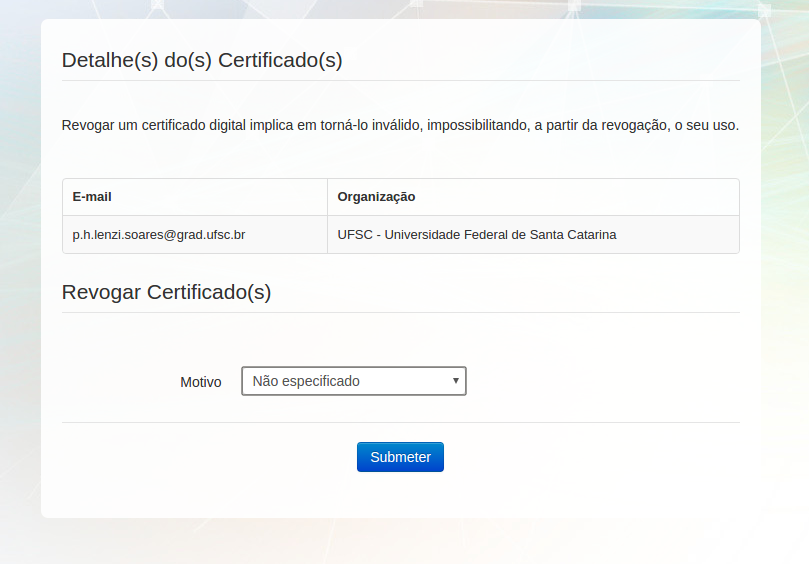
\includegraphics[scale=0.5]{images/saec21revoke.png}
     \caption{Página de revogação de certificado}
     \label{fig:revoke}
\end{figure}

\section{Ajuda}

No menu \textit{Ajuda} deve ser possível encontrar um guia que demonstra o passo a passo para todas as atividades do sistema, desde emissão do seu próprio certificado digital, até a configuração do cliente de e-mail. Basta clicar no menu e seguir as dicas da página. Os links posicionados na página devem levar o usuário exatamente à seção desejada.

\section{Repositório}

No menu \textit{Repositório do SAEC} deve ser possível encontrar o certificado da Autoridade Certificadora, que deverá ser automaticamente instalado no caso de o usuário utilizar o navegador Mozilla Firefox, ou precisa ser manualmente instalado, caso o usuário use Google Chrome, Internet Explorer ou Safari. Para acessar o guia de instalação, basta clicar no link \textit{Ajuda com a instalação}, posicionado ao lado do certificado a ser baixado. Teste a instalação nos quatro navegadores citados.

Deve ser possível também baixar a Lista de Certificados Revogados (LCR) da AC, apenas clicando no link disponibilizado nesta página. Para instalar a LCR, é necessário, novamente, clicar no link \textit{Ajuda com a instalação}, disponibilizado ao lado da LCR. Ambos os links de ajuda deverão redirecionar o usuário para a página de ajuda, apresentada na seção 6.2.

\section{Autenticação via Federação}

Quando autenticado perante uma federação, estará visível um campo informando que o usuário está autenticado, no canto direito da barra de menu. Ao clicar nessa barra, o usuário poderá ver as informações sobre ele que foram informadas pela federação, assim como ser instruído em como realizar o logoff da federação.